

%%%%%%%%%%%%%%%%%%%%%%%%%%%%%%%%%%%%%%%%%

%----------------------------------------------------------------------------------------
%	PACKAGES AND THEMES
%----------------------------------------------------------------------------------------

\documentclass{beamer}

\mode<presentation> {

% The Beamer class comes with a number of default slide themes
% which change the colors and layouts of slides. Below this is a list
% of all the themes, uncomment each in turn to see what they look like.

%\usetheme{default}
%\usetheme{AnnArbor}
%\usetheme{Antibes}
%\usetheme{Bergen}
%\usetheme{Berkeley}
%\usetheme{Berlin}
%\usetheme{Boadilla}
%\usetheme{CambridgeUS}
%\usetheme{Copenhagen}
%\usetheme{Darmstadt}
%\usetheme{Dresden}
%\usetheme{Frankfurt}
%\usetheme{Goettingen}
%\usetheme{Hannover}
%\usetheme{Ilmenau}
%\usetheme{JuanLesPins}
%\usetheme{Luebeck}
\usetheme{Madrid}
%\usetheme{Malmoe}
%\usetheme{Marburg}
%\usetheme{Montpellier}
%\usetheme{PaloAlto}
%\usetheme{Pittsburgh}
%\usetheme{Rochester}
%\usetheme{Singapore}
%\usetheme{Szeged}
%\usetheme{Warsaw}

% As well as themes, the Beamer class has a number of color themes
% for any slide theme. Uncomment each of these in turn to see how it
% changes the colors of your current slide theme.

%\usecolortheme{albatross}
%\usecolortheme{beaver}
%\usecolortheme{beetle}
%\usecolortheme{crane}
%\usecolortheme{dolphin}
%\usecolortheme{dove}
%\usecolortheme{fly}
%\usecolortheme{lily}
%\usecolortheme{orchid}
%\usecolortheme{rose}
%\usecolortheme{seagull}
%\usecolortheme{seahorse}
%\usecolortheme{whale}
%\usecolortheme{wolverine}

%\setbeamertemplate{footline} % To remove the footer line in all slides uncomment this line
%\setbeamertemplate{footline}[page number] % To replace the footer line in all slides with a simple slide count uncomment this line

%\setbeamertemplate{navigation symbols}{} % To remove the navigation symbols from the bottom of all slides uncomment this line
}

\usepackage{graphicx} % Allows including images
\usepackage{booktabs} % Allows the use of \toprule, \midrule and \bottomrule in tables
\usepackage[vietnamese]{babel}
%----------------------------------------------------------------------------------------
%	TITLE PAGE
%----------------------------------------------------------------------------------------

\title[Presentation ]{Đồ án \#2 - Xây dựng chương trình AI
} % The short title appears at the bottom of every slide, the full title is only on the title page

\author{ Đinh Đức Anh Khoa - 23122001 \\ Nguyễn Lê Hoàng Trung - 23122002 \\ Nguyễn Đình Hà Dương - 23122004 \\ Đinh Đức Tài - 23122013
} % 


\institute[23TNT1] % Your institution as it will appear on the bottom of every slide, may be shorthand to save space
{
FIT@HCMUS \\ % Your institution for the title page
\medskip
\textit{TPHCM, tháng 1 năm 2024} % 
}
\date{} % Date, can be changed to a custom date

\begin{document}

\begin{frame}
\titlepage % Print the title page as the first slide
\end{frame}

\begin{frame}
\frametitle{Tổng quan} % Table of contents slide, comment this block out to remove it
\tableofcontents % Throughout your presentation, if you choose to use \section{} and \subsection{} commands, these will automatically be printed on this slide as an overview of your presentation
\end{frame}

%----------------------------------------------------------------------------------------
%	PRESENTATION SLIDES
%----------------------------------------------------------------------------------------
\section{Mở đầu} 

\begin{frame}
\frametitle{1. Mở đầu}
\begin{itemize}
    \item Ở bài thuyết trình này, chúng ta sẽ tìm hiểu cách xây dựng mô hình neural network để giải quyết một bài toán cụ thể.
\end{itemize}
\end{frame}



\section{Bài toán cần giải quyết} 

\begin{frame}
\frametitle{2. Bài toán cần giải quyết}
\begin{itemize}
    \item \textbf{Bài toán:} Nhận diện các chữ số viết tay.
    \item \textbf{Sơ lược về mô hình:} Mô hình nhận đầu vào (input) là hình ảnh có kích thước \textbf{28x28 pixel} chứa một chữ số bất kỳ từ \textbf{0 đến 9}, sau đó dự đoán và đưa ra kết quả là một số nguyên tương ứng với chữ số xuất hiện trong hình ảnh nhận được ban đầu.
\end{itemize}
\end{frame}


\section{Dữ liệu và phân chia dữ liệu} 

\begin{frame}
\frametitle{3. Dữ liệu và phân chia dữ liệu}
- Dữ liệu được sử dụng trong mô hình này là tập dữ liệu \textbf{MNIST} được lấy từ website kaggle.com bao gồm 4 file:
\begin{figure}
    \centering
    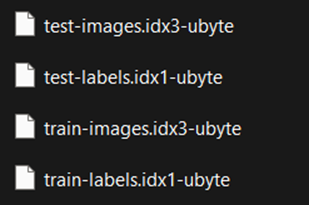
\includegraphics[width=0.5\linewidth]{images/dataset.png}
    \caption{Các tập dữ liệu}
\end{figure}
\end{frame}

\begin{frame}
\frametitle{3. Dữ liệu và phân chia dữ liệu}
\begin{figure}
    \centering
    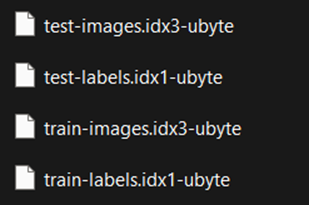
\includegraphics[width=0.3\linewidth]{images/dataset.png}
\end{figure}
    \begin{itemize}
    \item File \texttt{test-images.idx3-ubyte} chứa 60.000 hình ảnh có kích thước 28x28 pixel là các chữ số viết tay của tập huấn luyện (train set).
    \item File \texttt{train-labels.idx1-ubyte} chứa các nhãn là các chữ số tương ứng với từng hình ảnh của tập huấn luyện.
    \item File \texttt{test-images.idx3-ubyte} chứa 10.000 hình ảnh có kích thước 28x28 pixel là các chữ số viết tay của tập kiểm tra (test set).
    \item File \texttt{test-labels.idx1-ubyte} chứa các nhãn là các chữ số tương ứng với từng hình ảnh của tập kiểm tra.
\end{itemize}
\end{frame}

\begin{frame}
\frametitle{3. Dữ liệu và phân chia dữ liệu}
- Các hình ảnh trong tập dữ liệu đều có nền là màu đen và nét màu trắng thể hiện một chữ số bất kỳ từ 0 đến 9
\begin{figure}
    \centering
    
\includegraphics[width=0.3\linewidth]{images/data_sample.png}
    \caption{Ví dụ một hình ảnh của tập dữ liệu thể hiện chữ số 3}
\end{figure}
\end{frame}

\begin{frame}
\frametitle{3. Dữ liệu và phân chia dữ liệu}
- Tiếp theo, sử dụng phương thức \texttt{train\_test\_split} từ thư viện \texttt{scikit-learn} lên train set để tạo ra được một tập dữ liệu mới là validation set. Lúc này, train set sẽ được tách ra thành hai tập ngẫu nhiên với 5\% là validation set và phần còn lại là train set.
\\- Vậy ta sẽ có được ba tập dữ liệu sẽ được sử dụng cho các bước sau của mô hình:
\begin{itemize}
    \item \textbf{Train set}:  Sử dụng để huấn luyện và tinh chỉnh các tham số của mô hình.
    \item \textbf{Validation set}: Sử dụng để kiểm tra độ chính xác của mô hình trong quá trình học xem mô hình có thích nghi tốt với tập dữ liệu chưa từng thấy bao giờ hay không, từ đó có thể giảm thiểu vấn đề overfitting.
    \item \textbf{Test set}: Sử dụng để kiểm tra độ hiệu quả của mô hình sau khi được huấn luyện.
\end{itemize}
\end{frame}


\section{Thiết kế, huấn luyện mạng neutral} 

\begin{frame}
\frametitle{4. Thiết kế, huấn luyện neural network}
\begin{itemize}
    \item Kiến trúc neural network
    \item Lan truyền tiến, lan truyền ngược
    \item Loss function
    \item Optimizer
    \item Learning rate, số epoch, batch-size, regularization
    \item Độ chính xác và những vấn đề khác
\end{itemize}
\end{frame}

\subsection{Kiến trúc neural network} 

\begin{frame}
\frametitle{4.1 Kiến trúc neural network}
\begin{figure}
    \centering
    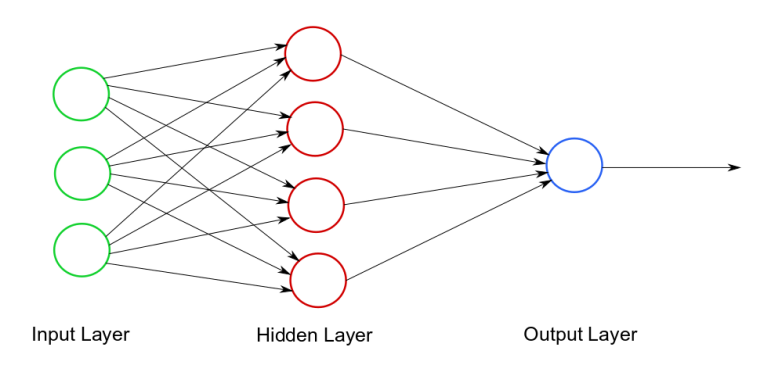
\includegraphics[width=1\linewidth]{images/neuralnet-visible.png}
    \caption{Mô hình neural network}
\end{figure}
\end{frame}

\begin{frame}
\frametitle{4.1 Kiến trúc neural network}
Kiến trúc: Mô hình neural network được sử dụng là một multilayer perceptron gồm một lớp đầu vào (input layer), một lớp ẩn (hidden layer) và một lớp đầu ra (output layer). 
    \begin{itemize}
    \item Input layer: Gồm 784 nút, mỗi nút thể hiện một pixel trên ma trận ảnh 28x28
    \item Hidden layer(s): Mô hình này sẽ chỉ gồm 1 lớp ẩn duy nhất gồm 10 nút. Dữ liệu từ lớp Input sẽ thông qua hàm Linear và hàm ReLu để tính toán kết quả đầu ra cho lớp ẩn. 
    \item Output Layer: Gồm 10 nút thể hiện các chữ số từ 0 đến 9. Kết quả đầu ra từ lớp ẩn sẽ thông qua hàm Linear để có được kết quả đầu ra cho lớp Output. Giá trị của mỗi nút là xác suất mà hình ảnh ban đầu chứa chữ số tương ứng mà nút đó thể hiện. Kết quả dự đoán của mô hình là nút có xác suất cao nhất. 
    \end{itemize}
\end{frame}

\subsection{Lan truyền tiến, lan truyền ngược} 
\begin{frame}
\frametitle{4.2 Lan truyền tiến và lan truyền ngược}
\begin{figure}
    \centering
    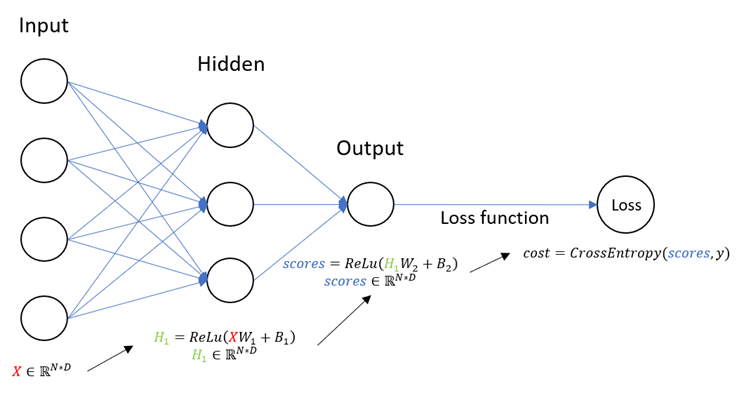
\includegraphics[width=1\linewidth]{images/forward.png}
    \caption{Mô hình mô phỏng lan truyền tiến}
\end{figure}
\end{frame}

\begin{frame}
\frametitle{4.2 Lan truyền tiến và lan truyền ngược}
\begin{figure}
    \centering
    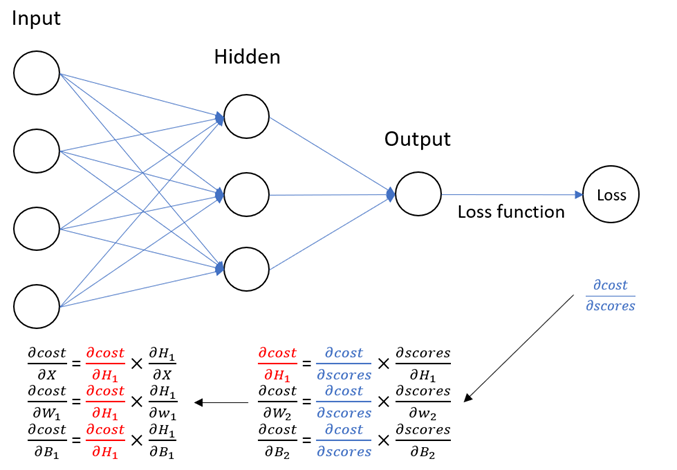
\includegraphics[width=0.8\linewidth]{images/backpro.png}
    \caption{Mô hình mô phỏng lan truyền ngược}
    
\end{figure}
\end{frame}

\begin{frame}
\frametitle{4.2 Lan truyền tiến và lan truyền ngược}
\begin{figure}
    \centering
    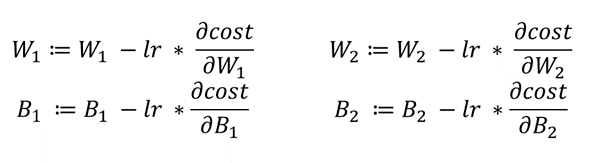
\includegraphics[width=1\linewidth]{images/update_w_b.png}
    \caption{Công thức cập nhật tham số (Weight và Bias) của từng lớp.}
    
\end{figure}
\end{frame}

\subsection{Loss function: CE và hàm Softmax} 

\begin{frame}
\frametitle{4.3 Loss function: CE và hàm Softmax}
- Đối với mô hình này, kết quả đầu ra của lớp Output có thể là các giá trị âm. Do đó, ta không thể trực tiếp sử dụng các giá trị này để tính toán sai số thông qua hàm Cross-Entropy được. Thay vào đó ta sẽ \textbf{chuẩn hóa các giá trị này bằng hàm Softmax} có hai tính chất là các xác suất luôn nằm trong khoảng (0, 1] và tổng các xác suất bằng 1. Sau đó sử dụng các giá trị đã chuẩn hóa này để tính toán sai số thông qua hàm Cross-Entropy. 
\\- Giả sử có một vector đầu vào $z = (z_1, z_2, ..., z_k)$, hàm Softmax sẽ tính xác suất $p_i$ cho mỗi phần tử theo công thức:
\begin{center}
    \Large $p_{i}=\frac{e^{z_{i}}}{\sum_{j=1}^{k}e^{z_{j}}},\forall i=1,2,...,k$
\end{center}
\end{frame}

\begin{frame}
\frametitle{4.3 Loss function: CE và hàm Softmax}
\textbf{Cross-Entropy Loss function:}
    \begin{center}
        \large $CE = - \sum_{i=1}^{C} P_{i}\times \log(Q_{i})$
    \end{center}
    Trong đó:
    \begin{itemize}
        \item $C$: số lượng các class cần phân lớp.
        \item $Q_{i}$: xác suất thực tế của lớp thứ i
        \item $P_{i}$: xác suất dự đoán của lớp thứ i bởi mô hình
    \end{itemize}
\end{frame}

\subsection{Optimizer} 

\begin{frame}
\frametitle{4.4 Optimizer}
\begin{figure}
    \centering
    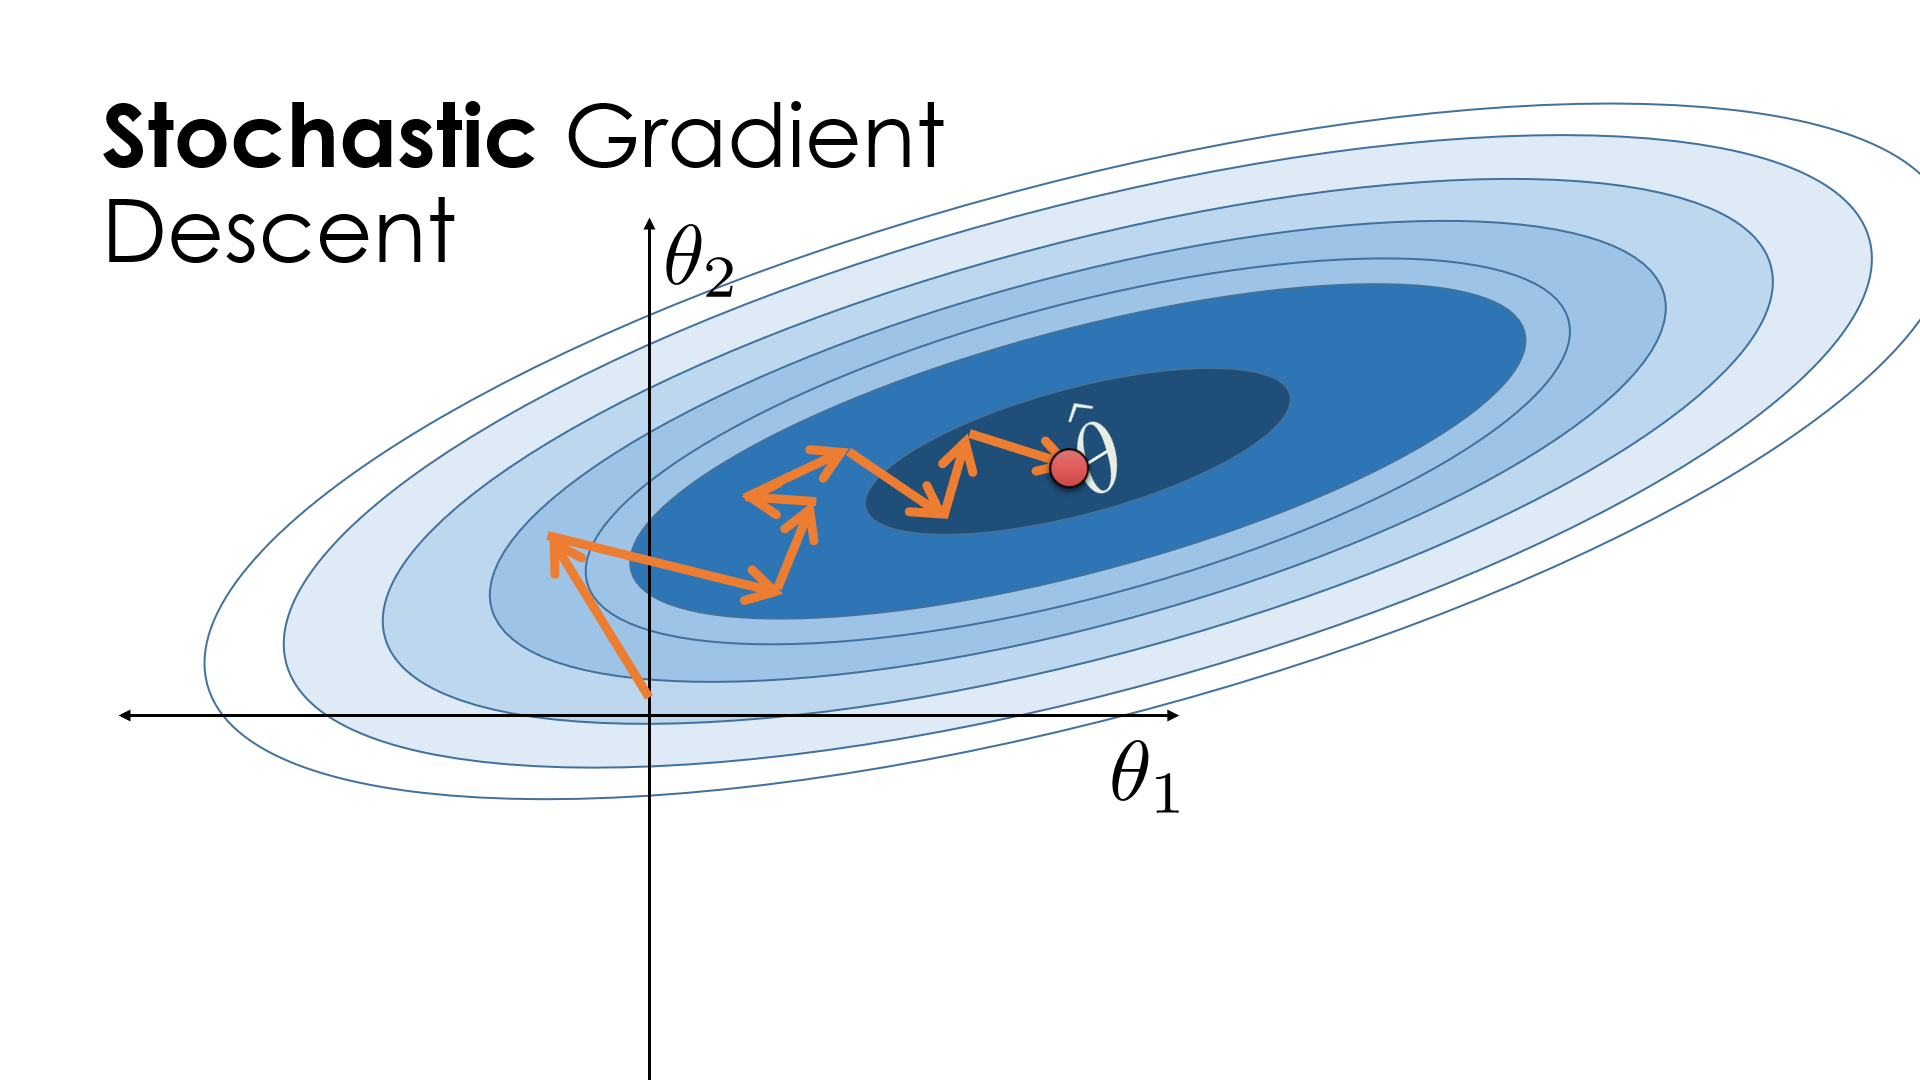
\includegraphics[width=1\linewidth]{images/SGD.png}
    \caption{Stochastic Gradient Descent}
    
\end{figure}
\end{frame}

\subsection{Learning rate, số epoch, batch-size, regularization} 

\begin{frame}
\frametitle{4.5 Learning rate, số epoch, batch-size, regularization}
\begin{itemize}
    \item \textbf{Learning rate:} 
\end{itemize}
    \\- Ban đầu khởi tạo giá trị \texttt{learning\_rate} thủ công, cứ sau mỗi \texttt{decay\_after} lần lặp thì ta sẽ cập nhật giá trị \texttt{learning\_rate} mới bằng cách nhân với một lượng \texttt{learning\_rate\_decay} (với \texttt{learning\_rate\_decay} < 1). 
    \\- Điều này sẽ giúp tăng dần tính chính xác với \texttt{learning\_rate} giảm dần khi tiến lại gần điểm hội tụ, tránh trường hợp \texttt{learning\_rate} quá lớn dẫn đến việc phân kì. 
    \begin{itemize}
        \item $learning\_rate = 0.001$
        \item $decay\_after = 50$
        \item $learning\_rate\_decay = 0.99$
    \end{itemize}
    
\end{frame}

\begin{frame}
\frametitle{4.5 Learning rate, số epoch, batch-size, regularization}
\begin{itemize}
 \item \textbf{Số epoch:} Số lần truyền tập train để huấn luyện cho neural network
    \begin{itemize}
        \item $epoch = 200$
    \end{itemize}
    \item \textbf{Batch-size:} Tách bộ dữ liệu train thành các batch nhỏ hơn với kích thước là \texttt{batch-size} để tối ưu tốc độ huấn luyện.
    \begin{itemize}
        \item $batch-size = 200$
    \end{itemize}
    \item \textbf{Regularization:} Hằng số được thêm vào quá trình tính gradient để giảm hiện tượng
overfitting 
    \begin{itemize}
        \item $Regularization = 5\times 10^{-6}$
    \end{itemize}
\end{itemize}
    
\end{frame}

\section{Quá trình hội tụ, kết quả kiểm thử mô hình} 

\begin{frame}
\frametitle{5. Quá trình hội tụ, kết quả kiểm thử mô hình}
\begin{itemize}
    \item Trong quá trình huấn luyện, giá trị của hàm loss (average cost) giảm dần và độ chính xác của train set và validation set tăng dần theo số lần lặp (epoch).
    \item Trong quá trình huấn luyện, ở \textbf{epoch cuối}:
    \begin{itemize}
        \item Giá trị cost trung bình: 0.36
        \item Độ chính xác (accuracy) trên train set: 89\%
        \item Độ chính xác (accuracy) trên validation set: 89\%
    \end{itemize}
    \item \textbf{Trong quá trình kiểm thử mô hình, độ chính xác (accuracy) trên test set: 89\%}
    \begin{figure}
        \centering
        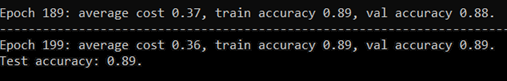
\includegraphics[width=1\linewidth]{images/testacc.png}
        \caption{Accuracy - test set}
        
    \end{figure}
\end{itemize}
\end{frame}

\section{Demo} 

\begin{frame}
\frametitle{6. Demo}
\begin{itemize}
    \item 4 hình ảnh trong test set mà mô hình dự đoán đúng
    \begin{figure}[H]
    \centering
    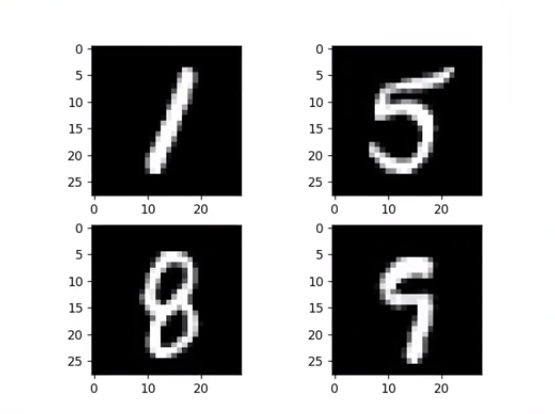
\includegraphics[width=0.75\linewidth]{images/true.png}
    \caption{Các mẫu mô hình dự đoán đúng}
        
    \end{figure}
    
\end{itemize}
\end{frame}

\begin{frame}
\frametitle{6. Demo}
\begin{itemize}
\item 4 hình ảnh trong test set mà mô hình dự đoán sai
    \begin{figure}[H]
    \centering
    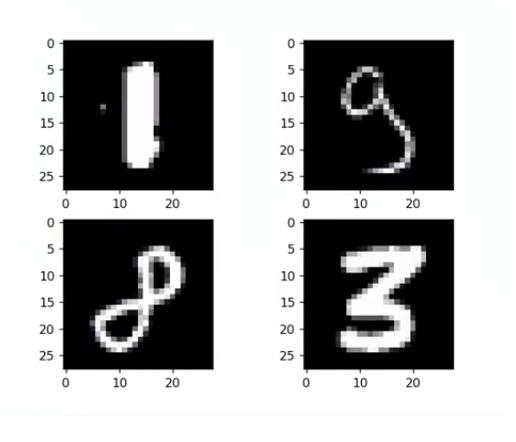
\includegraphics[width=0.75\linewidth]{images/false.png}
    \caption{Các mẫu mô hình dự đoán sai}
\end{figure}
\end{itemize}
\end{frame}

\begin{frame}
\frametitle{Tham Khảo}

\begin{itemize}
    \item The MNIST database of handwritten digits \\https://www.kaggle.com/datasets/hojjatk/mnist-dataset
    \item MLP Neural Network \\https://github.com/SonPhatTran/Neural-Network-from-scratch
    \item Demo 
    \\https://www.youtube.com/watch?v=UQExhzgt-6E
\end{itemize}


\end{frame}

\begin{frame}
\Huge{\centerline{The End}}
\end{frame}

%----------------------------------------------------------------------------------------

\end{document} 